\documentclass{beamer}
\usepackage{xcolor}
\graphicspath{{media/}}
\usepackage{tikz}
\usetikzlibrary{fit, backgrounds, shapes, arrows, arrows.meta, chains}

\usepackage[outputdir=/tmp/latexrun]{minted}
\newminted{javascript}{
    autogobble,
    breaklines,
    linenos,
    fontsize=\footnotesize,
    framesep=2mm,
    frame=lines}
\newmintinline{javascript}{}

% Suppress navigation bar
\beamertemplatenavigationsymbolsempty

\mode<presentation> {
    \usetheme{unipassau}
    \setbeamercovered{transparent}
}

\logo{}

% Title slide definition
\title[Whisker: Automated Testing of Scratch Programs]{Whisker: Automated Testing\\of Scratch Programs}
\subtitle{}
\author{Marvin Kreis}
\institute {
    Chair of Software Engineering II\\
    University of Passau
}
\date{2019-03-27}

\newcommand{\bigcenter}[1]{
    \begin{center}
        \textcolor{black!70}{\Huge #1}
    \end{center}
}


%--------------------------------------------------------------------
% Titlepage
%--------------------------------------------------------------------

\begin{document}

\setbeamertemplate{footline}[default]

\begin{frame}
    \titlepage
\end{frame}

\setbeamertemplate{footline}[unipassautheme]



%-------------------------------------------------------------------
% Content
%-------------------------------------------------------------------

% \begin{frame}\frametitle{Frametitle 1}
%
%     \begin{block}{Definition}
%         This is a definition.
%     \end{block}
%     \begin{columns}[t]
%     \column{5cm}
%     \begin{itemize}
%         \item \textcolor{uporange}{uporange}
%         \item \textcolor{upgrey}{upgrey}
%         \item \textcolor{upjura}{upjura}
%         \item \textcolor{upphil}{upphil}
%         \item \textcolor{upwiwi}{upwiwi}
%         \item \textcolor{upfim}{upfim}
%     \end{itemize}
%     \column{5cm}
%     \begin{enumerate}
%         \item Element 1
%         \item Element 2
%     \end{enumerate}
%     \end{columns}
%
% \end{frame}
%
% \begin{frame}\frametitle{Frametitle 2}
%
%     \begin{table}[ht!]
%     \centering
%     \begin{tabular}{|lccc|}
%         \hline
%         Name & Mat. Nr. & Semester & Degree Course \\
%         \hline
%         Example 1 & 1234 & 10 & M.Sc. BA\\
%         Example 2 & 4567 & 8 & M.Sc. CS \\
%         Example 3 & 7890 & 5 & B.A. ES \\
%         Example 4 & 9012 & 4 & B.Sc. IC \\
%         \hline
%     \end{tabular}
%     \caption{Students}
%     \end{table}
%
% \end{frame}

\begin{frame}
    \bigcenter{What is Scratch?}
\end{frame}

\begin{frame}\frametitle{What is Scratch?}
    \begin{figure}
        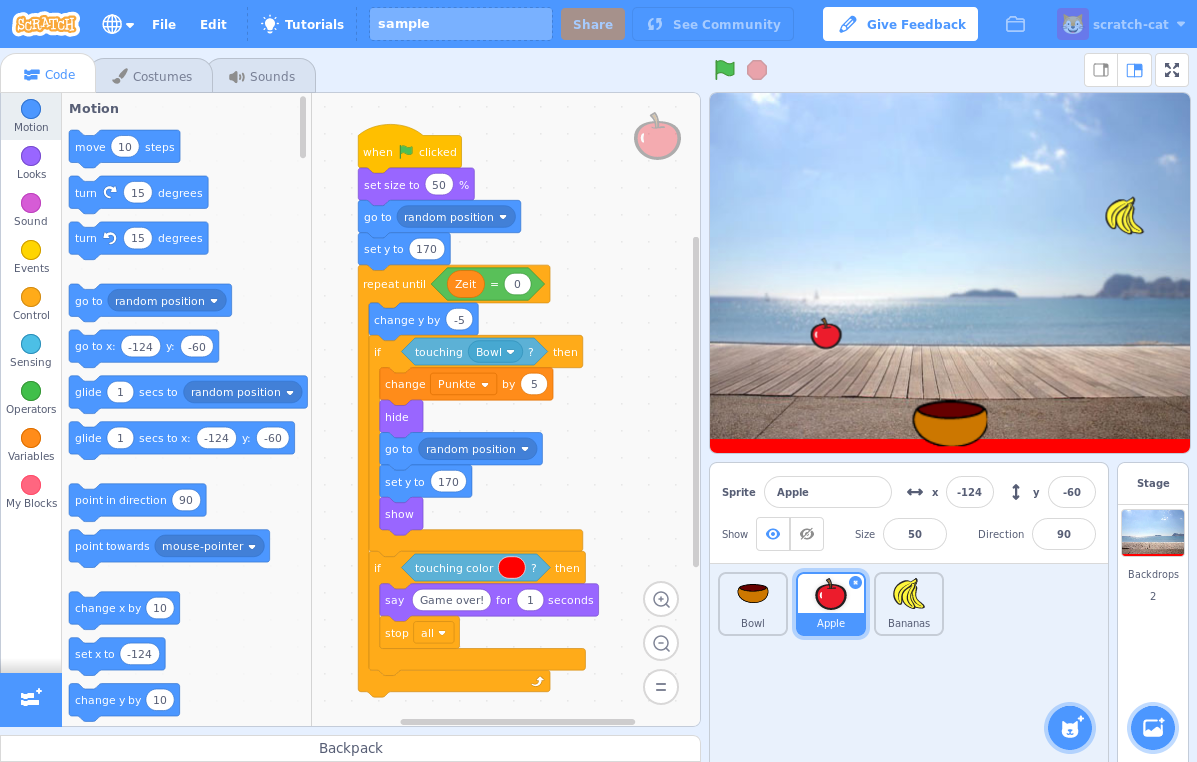
\includegraphics[width=.9\textwidth]{scratch-gui}
        \caption{Scratch's GUI}
    \end{figure}
\end{frame}

\begin{frame}\frametitle{What is Scratch?}
    \begin{itemize}
        \item Block-based programming language
        \item Developed by the MIT media lab
        \item Code is separated into scripts that are triggered by events
    \end{itemize}

    \begin{figure}
        \centering
        \tikzset{>=latex,
                 arrow/.style={-{Latex[length=1.5mm, width=1.5mm]}},
                   box/.style={draw, text width=3.2cm, minimum height=0.7cm, text centered, rounded corners},
                 label/.style={text width=1.9cm}}

        \begin{tikzpicture}[scale=0.8, every node/.style={scale=0.8}]
            \node[box] at (0.0, 1.5) (step)   {Run scripts in parallel until a sprite changes};
            \node[box] at (0.0, 0.0) (render) {Render the stage};

            \node[label] at (-3.5, 1.0) {30 times per second};

            \draw[shorten >= 2pt, arrow, rounded corners]
                   (step)
                -- (render)
                -- ( 0.0, -1.0)
                -- (-2.4, -1.0)
                -- (-2.4,  3.0)
                -- ( 0.0,  3.0)
                -- (step);
        \end{tikzpicture}

        \caption{Scratch step cycle}
    \end{figure}
\end{frame}

\begin{frame}
    \bigcenter{Why Scratch?}
    % Why is Scratch relevant?
    % Scratch is widely popular
    % For one thing, Scratch has a big online community
\end{frame}

\begin{frame}\frametitle{Why Scratch? Scratch's online community}
    % It has an online repository that everyone can upload their own projects to
    \begin{figure}
        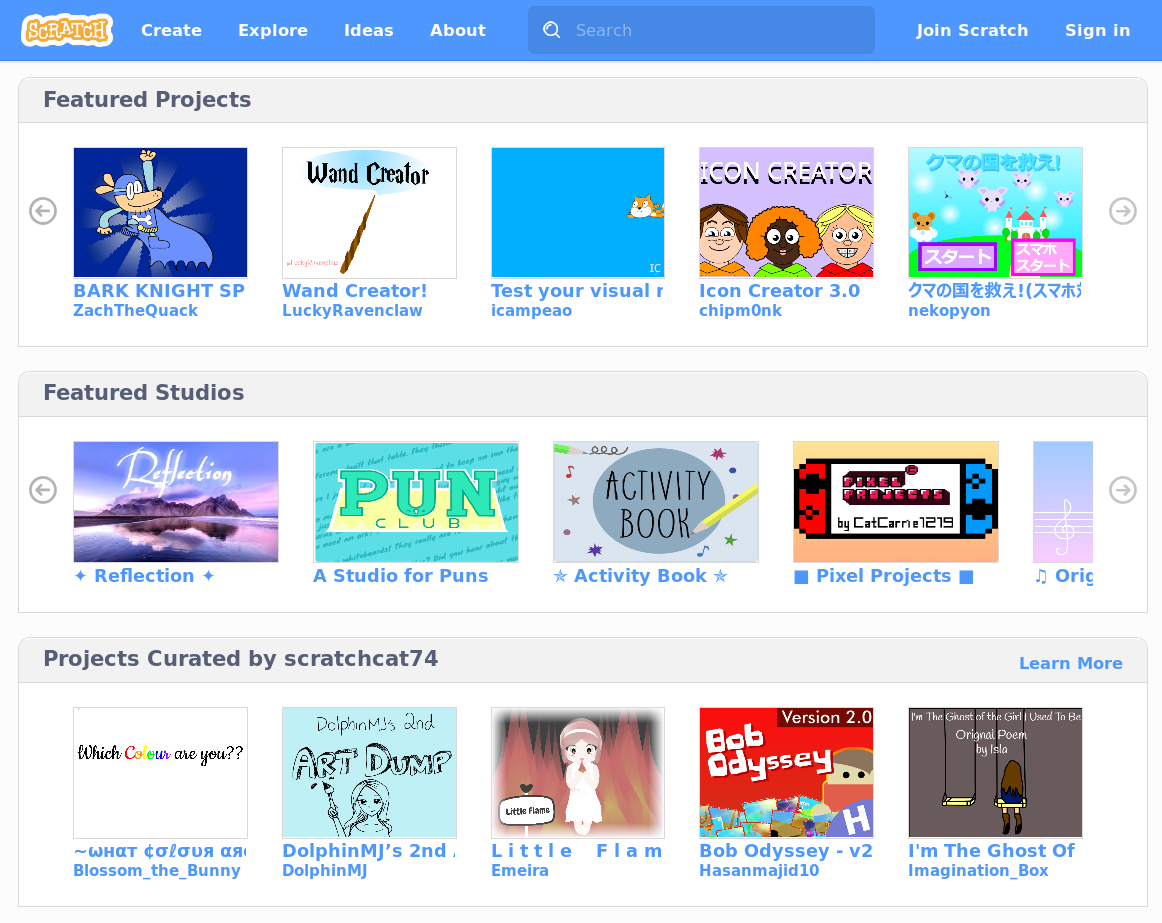
\includegraphics[width=.7\textwidth]{scratch-repository}
        \caption{Scratch's online repository}
    \end{figure}
\end{frame}

\begin{frame}[shrink=0]\frametitle{Why Scratch? Scratch's online community}
    % This repository encompasses over 38 million Scratch projects from over 36 million users at the time of writing
    % With over a million projects uploaded each month
    \begin{figure}
        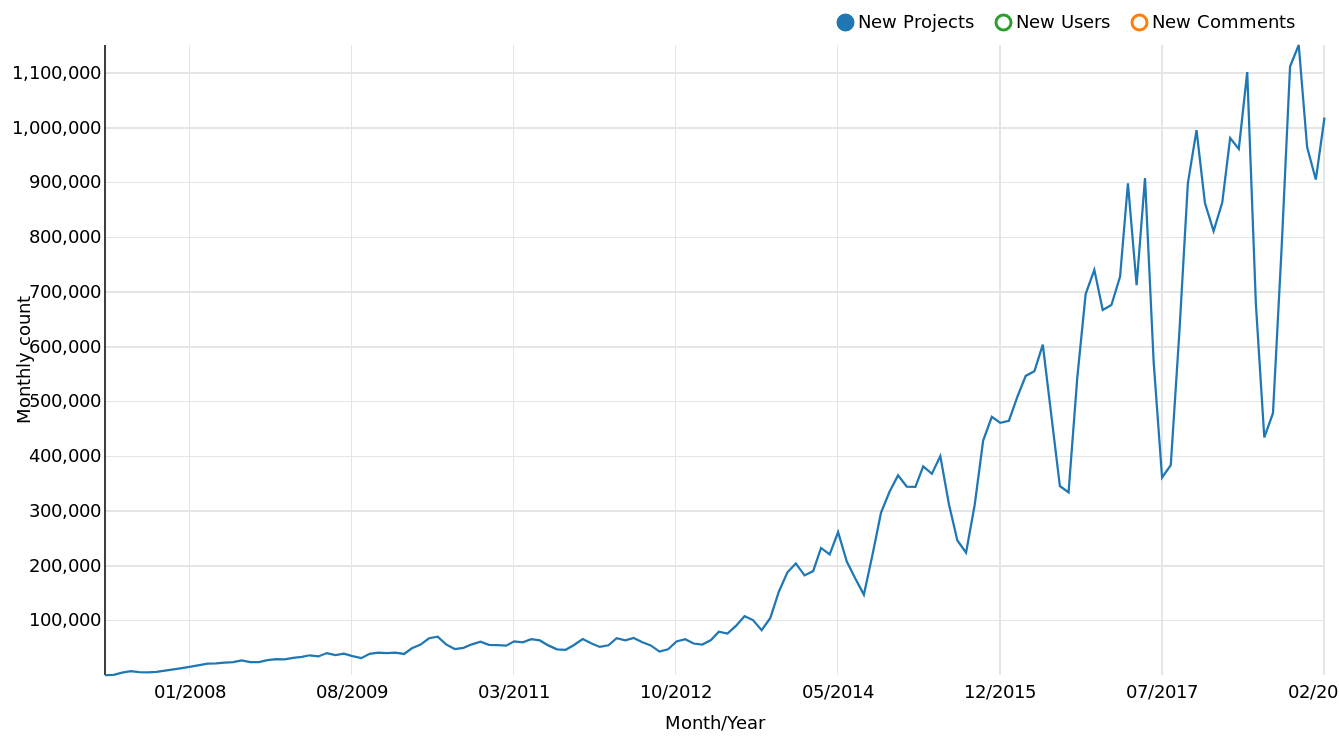
\includegraphics[width=.7\textwidth]{scratch-popularity}
        \caption{Submitted Scratch projects per month}
    \end{figure}
    \centering
    \begin{minipage}{.7\textwidth}
        \begin{itemize}
            \item over 38 million projects shared
            \item over 36 million users
        \end{itemize}
    \end{minipage}
\end{frame}

\begin{frame}\frametitle{Why Scratch? Good introduction to programming}
    % But more importantly Scratch is used by many schools and universities to introduce students to the principles of programming
    % Scratch is very suitable for this task for multiple reasons
    Many schools and universities deploy Scratch as a gentle introduction to programming.
\end{frame}

\begin{frame}\frametitle{Why Scratch? Good introduction to programming}
    % For one thing, Scratch makes it impossible to write invalid code
    % The block-based code system eliminates the possibility of syntax errors
    % Blocks are chosen from a drawer
    % And even variable names can't be misspelled since they are chosen from a list
    % This all helps make Scratch very intuitive to use
    \centering
    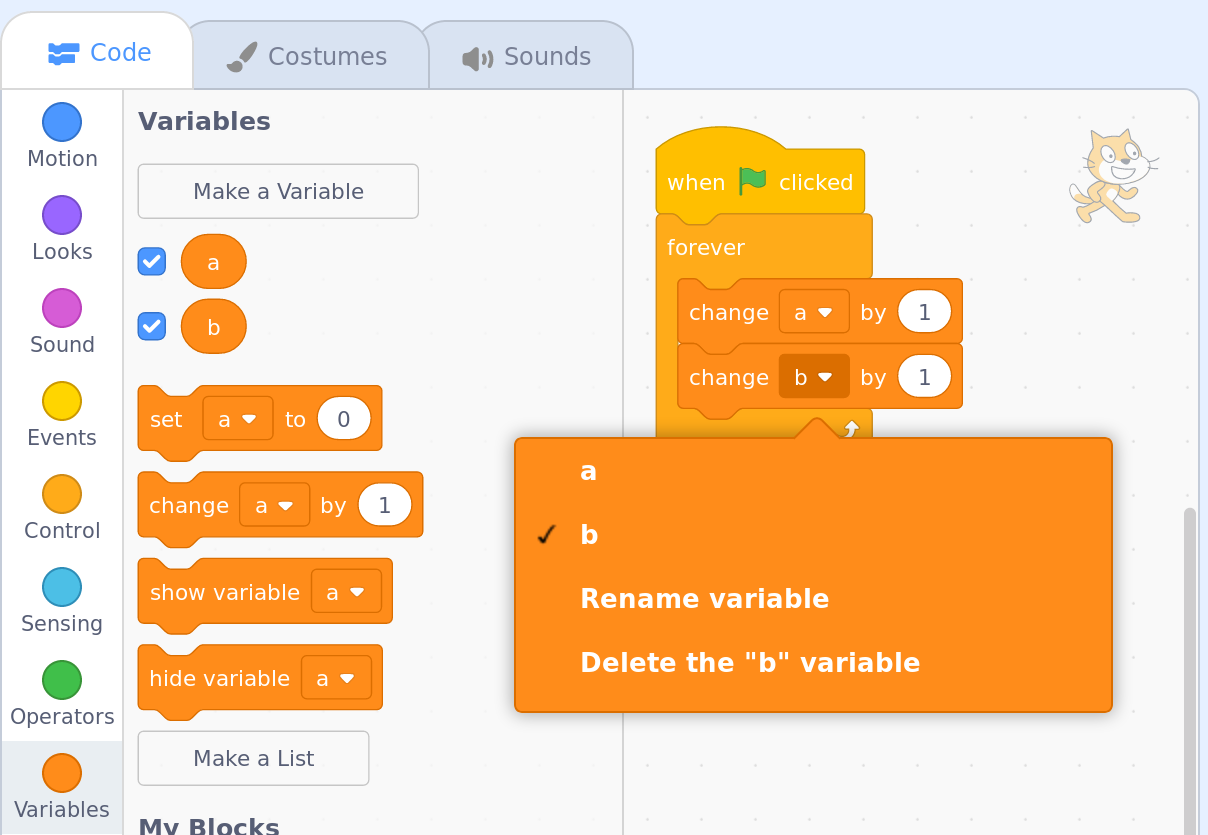
\includegraphics[width=.8\textwidth]{scratch-valid-code}\\[\medskipamount]
    Intuitive: Block based code system only allows valid code
\end{frame}

\begin{frame}\frametitle{Why Scratch? Good introduction to programming}
    % At the same time, Scratch is very engaging
    % User input, graphics and audio are easy to integrate, which often leads to game-like programs
    \centering
    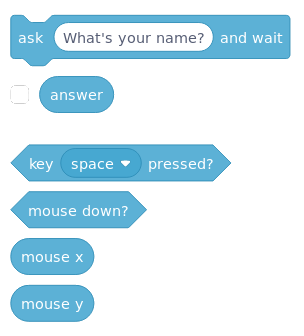
\includegraphics[width=.33\textwidth]{scratch-input-blocks}
    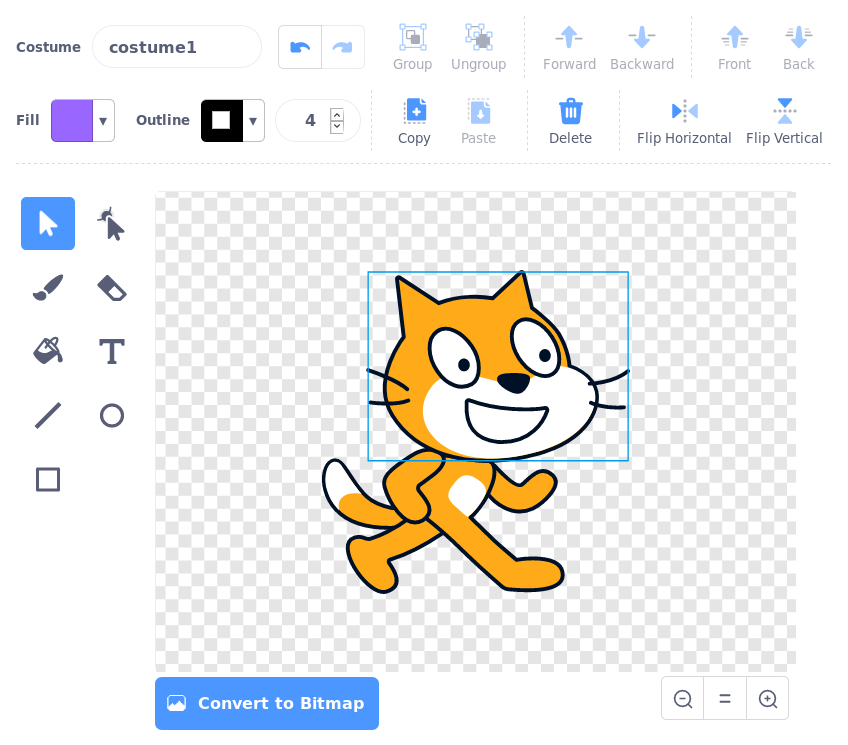
\includegraphics[width=.4\textwidth]{scratch-sprite-editor}
    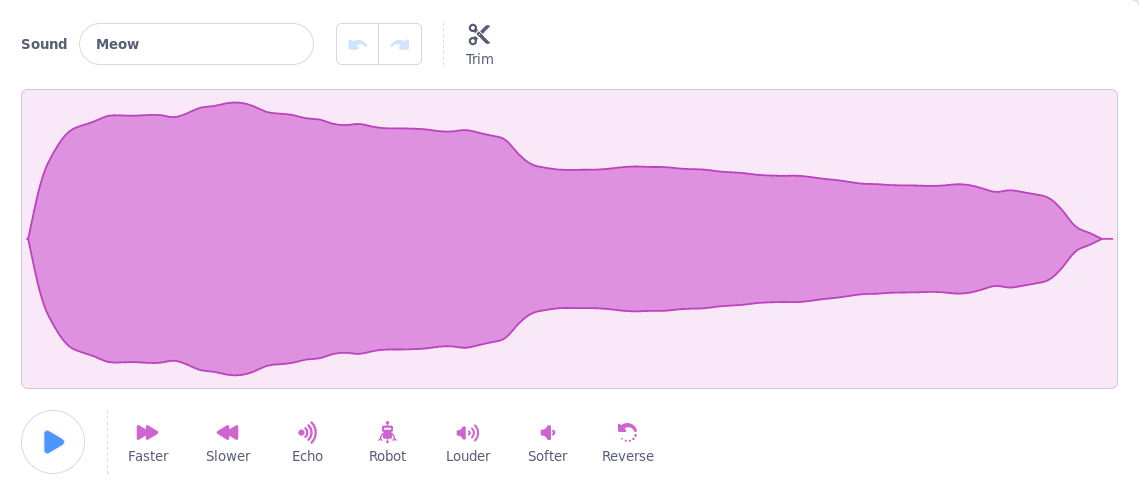
\includegraphics[width=.6\textwidth]{scratch-sound-editor}\\[\medskipamount]
    Engaging: User interaction, easy integration of graphics and sounds
\end{frame}

\begin{frame}
    \bigcenter{Why automated testing for Scratch?}
\end{frame}

\begin{frame}\frametitle{Why automated testing for Scratch?}
    Grading Scratch assignments is very \textcolor{upfim}{time consuming}
    \begin{itemize}
        \item every project has to be opened individually
        \item programs require large amounts of \textcolor{upfim}{user interaction}
    \end{itemize}

    \bigskip

    % TODO citation
    Some courses are attended by a \textcolor{upfim}{large number of students ($> 200$)},
    making manual testing for grading infeasible.

    \bigskip

    Students can also use automated tests to get feedback for their own implementations.
\end{frame}


\end{document}
